\chapter{Bausteinsicht}

\section{Ebene 1}

Der Machtpunktezähler besteht aus vier Subsystemen. Die gestrichelten Pfeile stellen Abhängigkeiten der Subsysteme untereinander dar (x -> y für x ist abhängig von y). Die Kästchen im Äußeren Rand bilden die Kommunikationspunkte mit anderen Systemen bzw. Nutzern.

\begin{figure}[h]
\begin{center}
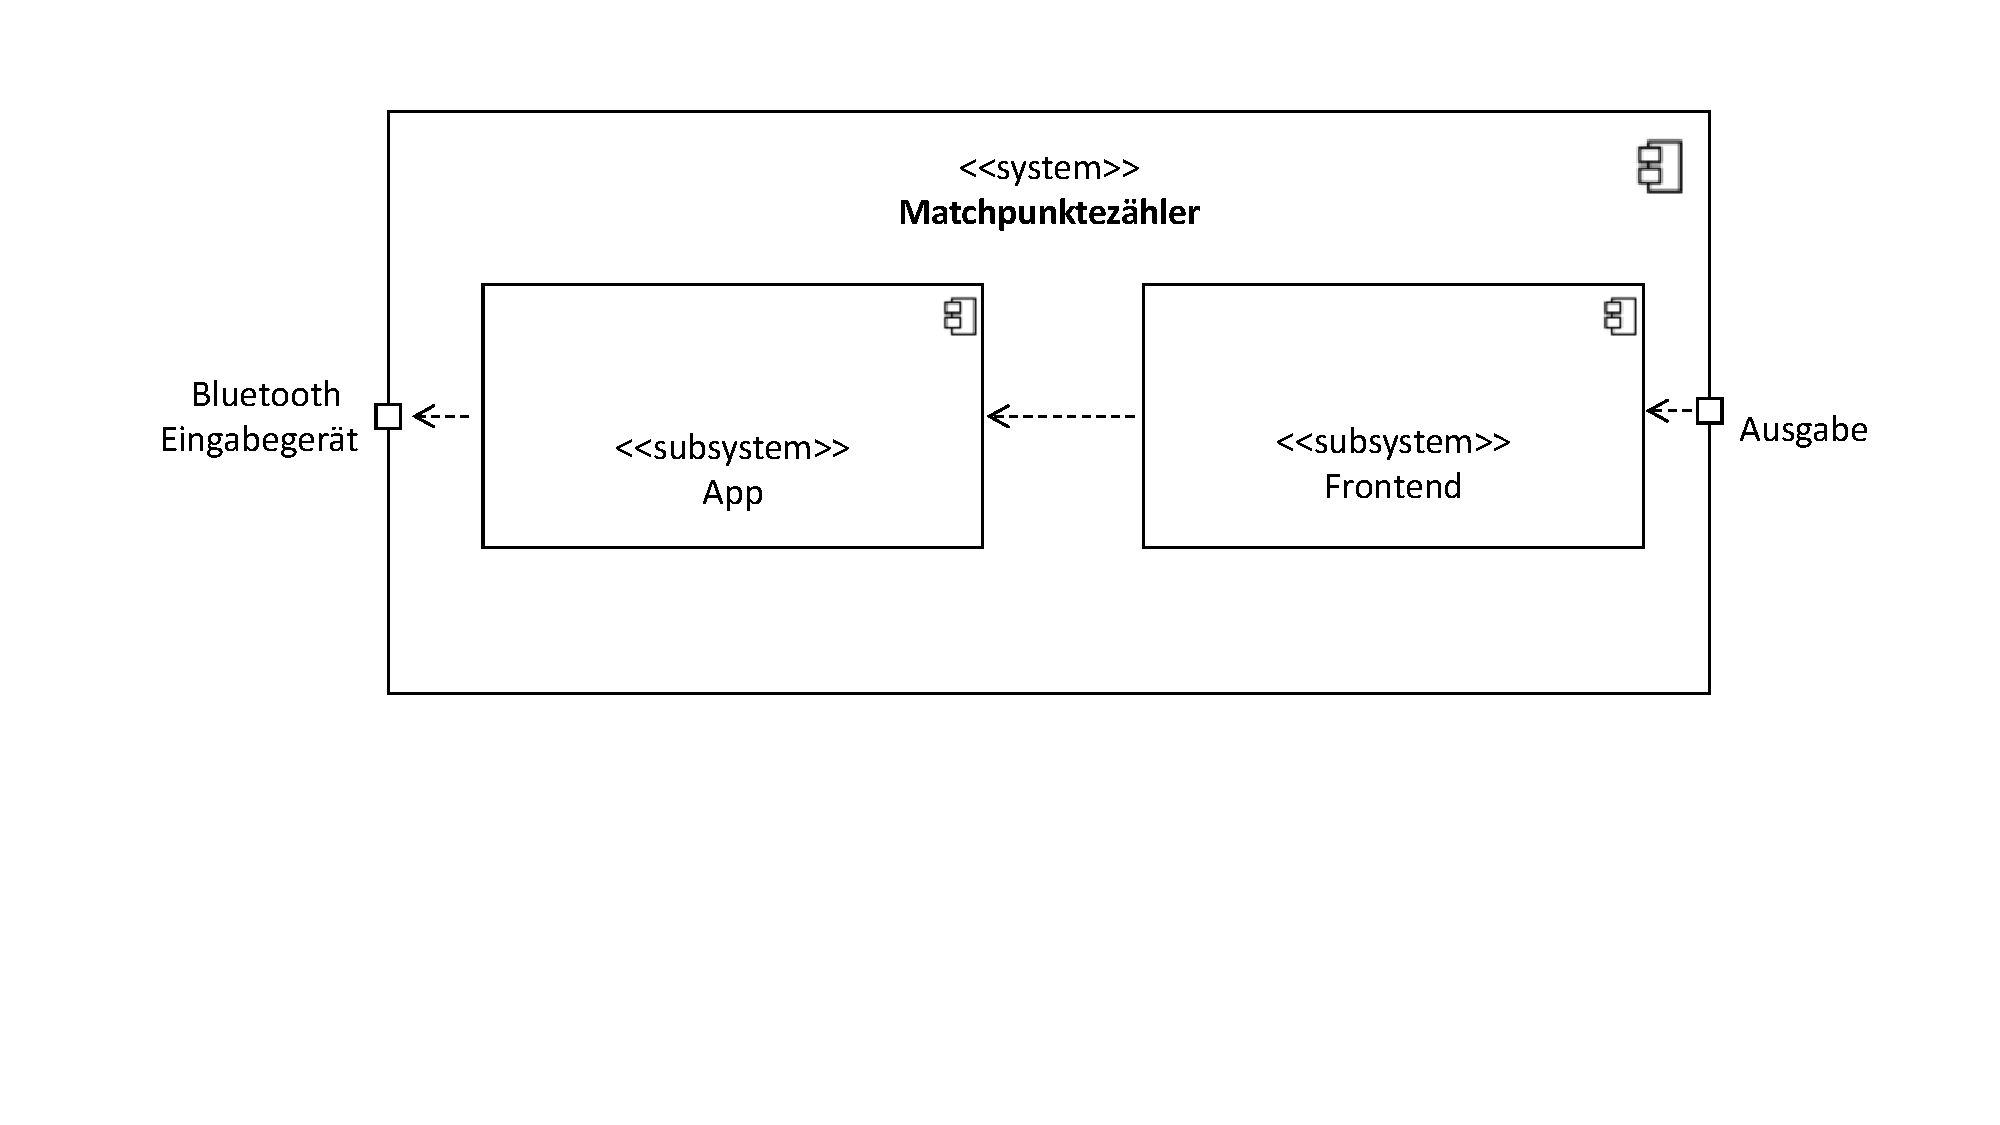
\includegraphics[scale=0.5]{Grafiken/Baustein_1.pdf}
\caption{Bausteinansicht Ebene 1}
\end{center}
\end{figure}

\begin{center}
\begin{tabular}[h]{|l|l|}
\cline{1-2}
\textbf{Subsystem} & \textbf{Kurzbeschreibung}\\
\cline{1-2}
Controller & Realisiert die Kommunikation, Verarbeitung der Eingaben\\&und Umsetzung der Spielregeln.\\ 
\cline{1-2}
Spielregeln & Beinhaltet die jeweiligen Spielregeln und macht es\\&möglich z.B. zu ermitteln wer Aufschlag hat.\\
\cline{1-2}
Bluetooth-Interface & Interpretiert die Bluetooth-Eingaben und verbindet neue Geräte.\\
\cline{1-2}
Frontend & Gibt anhand der vom Backend gegebenen Daten die Spielstand grafisch aus.\\
\cline{1-2} 
\end{tabular}
\end{center}

\section{Controller}
\subsection*{Zweck/Verantwortlichkeit}
Das Subsystem realisiert die Kommunikation zwischen den Subsystemen (z.B. mit dem Frontend). Bei einer Eingabe über das Subsystem Bluetooth-Interface werden über den Controller mit Hilfe der Spielregeln die Daten für die Ausgabe über das Frontend ermittelt.
\subsection*{Schnittstellen}
\subsection*{Ablageort / Datei}
\subsection*{Offene Punkte}

\section{Spielregeln}
\subsection*{Zweck/Verantwortlichkeit}
Das Subsystem bietet die Grundlage zur Funktionsweise des Systems. Es werden die Eingaben gemäß des Spielertypen interpretiert und in eine Ausgabe an das Frontend umgewandelt.
\subsection*{Schnittstellen}
Das Subsystem stellt seine Funktionalität über 
\begin{center}
\begin{tabular}[h]{|l|l|}
\cline{1-2}
\textbf{Methode} & \textbf{Kurzbeschreibung}\\
\cline{1-2}
CounterUp & Erhöht Spielstand für ein Team.\\ 
\cline{1-2}
Undo & Stellt den zuvor bestandenen Spielstand wieder her.\\
\cline{1-2}
Redo & Macht ein Undo wieder Rückgängig .\\
\cline{1-2}
UpdatePlayerPosition & Gibt die aktuellen Positionen der Spieler zurück.\\
\cline{1-2} 
UpdateServePosition & Gibt die Momentane Aufschlagposition zurück.\\
\cline{1-2}
\end{tabular}
\end{center}
\subsection*{Ablageort / Datei}
\subsection*{Offene Punkte}

\section{Bluetooth-Interface}
\subsection*{Zweck/Verantwortlichkeit}
Das Subsystem ist für das Verbinden und die Kommunikation mit einem Bluetooth-Eingabegerät verantwortlich. Somit wird am Anfang die Verbindung mit dem Eingabegerät hergestellt und anschließend bei einer Betätigung die Eingabe eingelesen und vor interpretiert.
\subsection*{Schnittstellen}
\subsection*{Ablageort / Datei}
\subsection*{Offene Punkte}

\section{Frontend}
\subsection*{Zweck/Verantwortlichkeit}
\subsection*{Schnittstellen}
\subsection*{Ablageort / Datei}
\subsection*{Offene Punkte}

\section{Ebene 2: App}

\begin{figure}[h]
\begin{center}
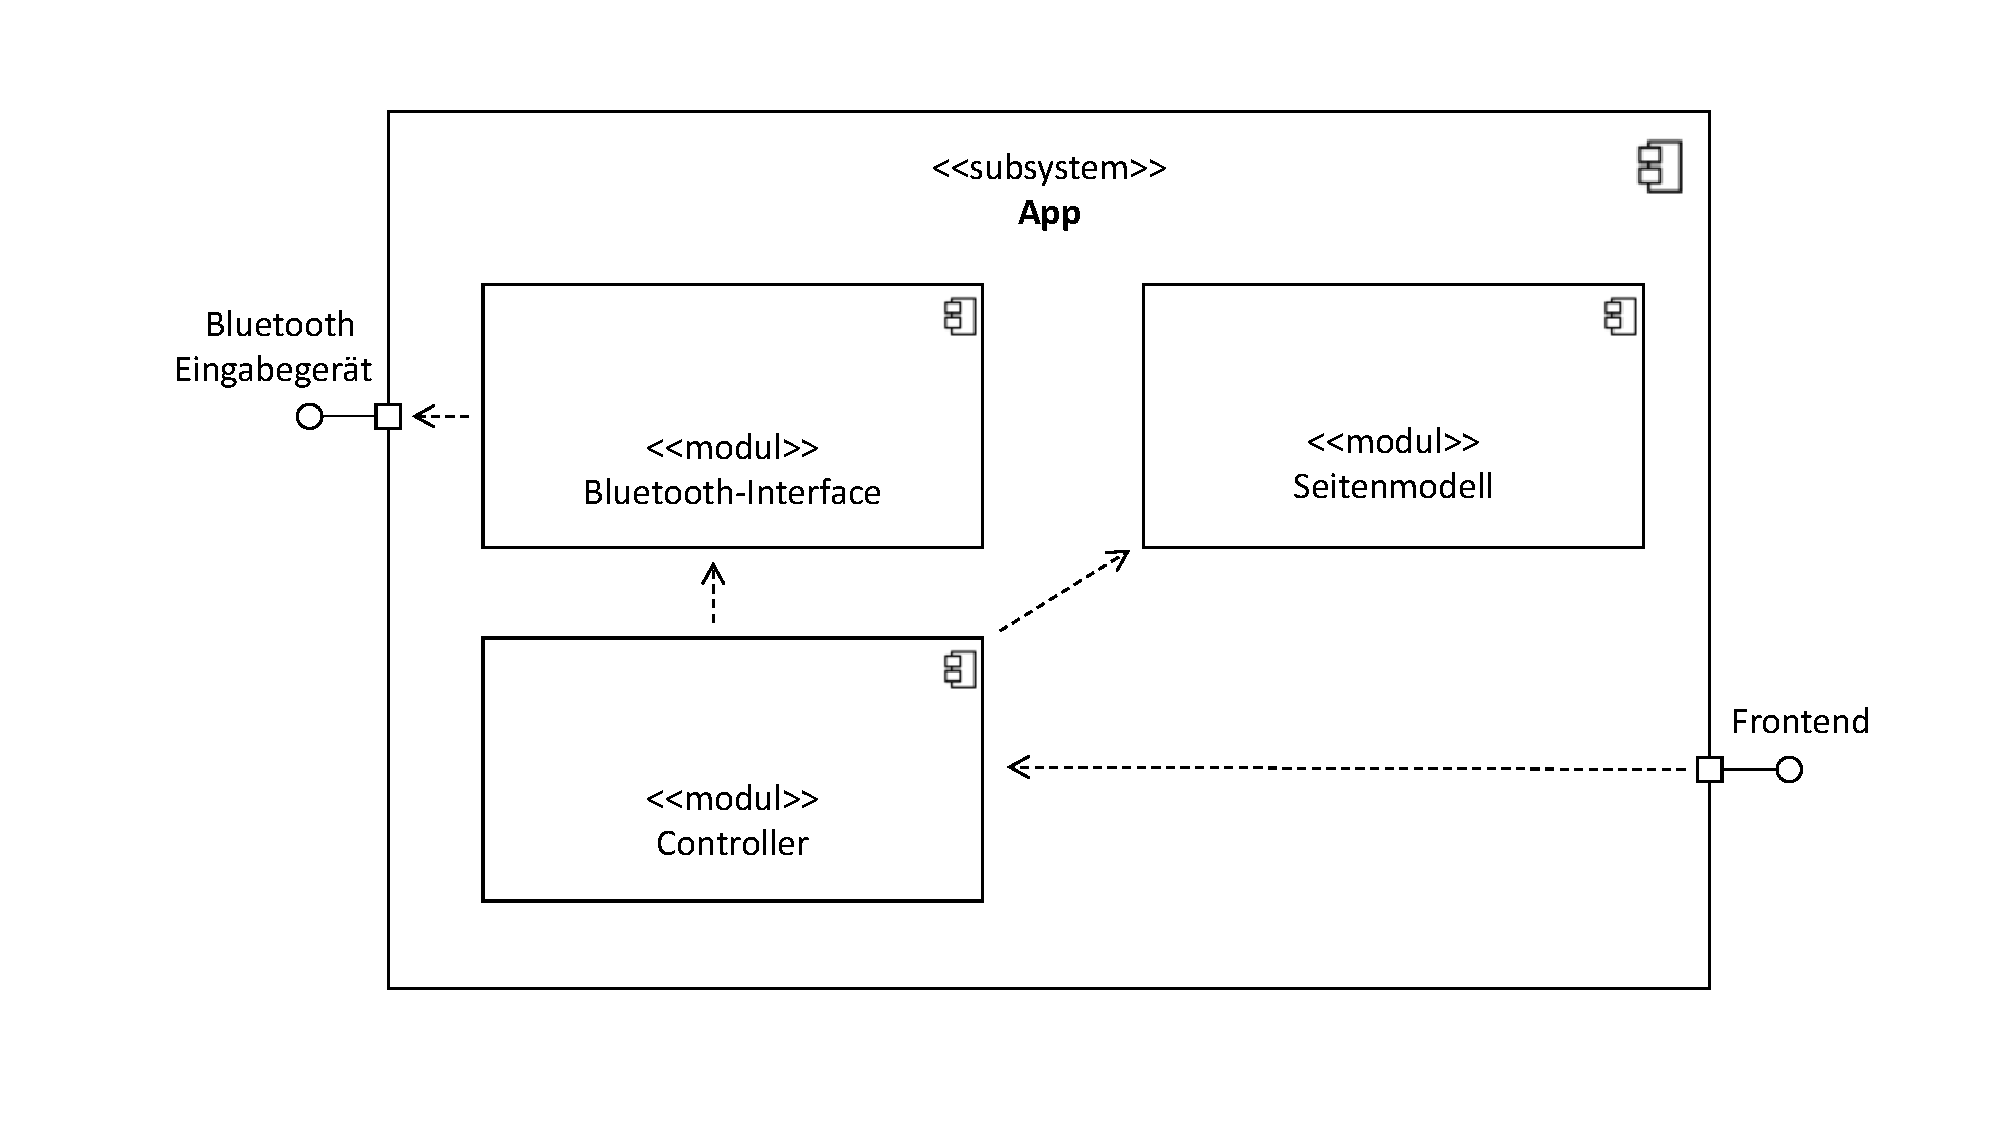
\includegraphics[scale=0.5]{Grafiken/Baustein_2.pdf}
\caption{Bausteinansicht Ebene 2: App}
\end{center}
\end{figure}